\documentclass{standalone}
\usepackage{tikz}
\usetikzlibrary{patterns, positioning}
\usepackage[sfdefault]{ClearSans} %% option 'sfdefault' activates Clear Sans as the default text font
\usepackage[T1]{fontenc}

\begin{document}
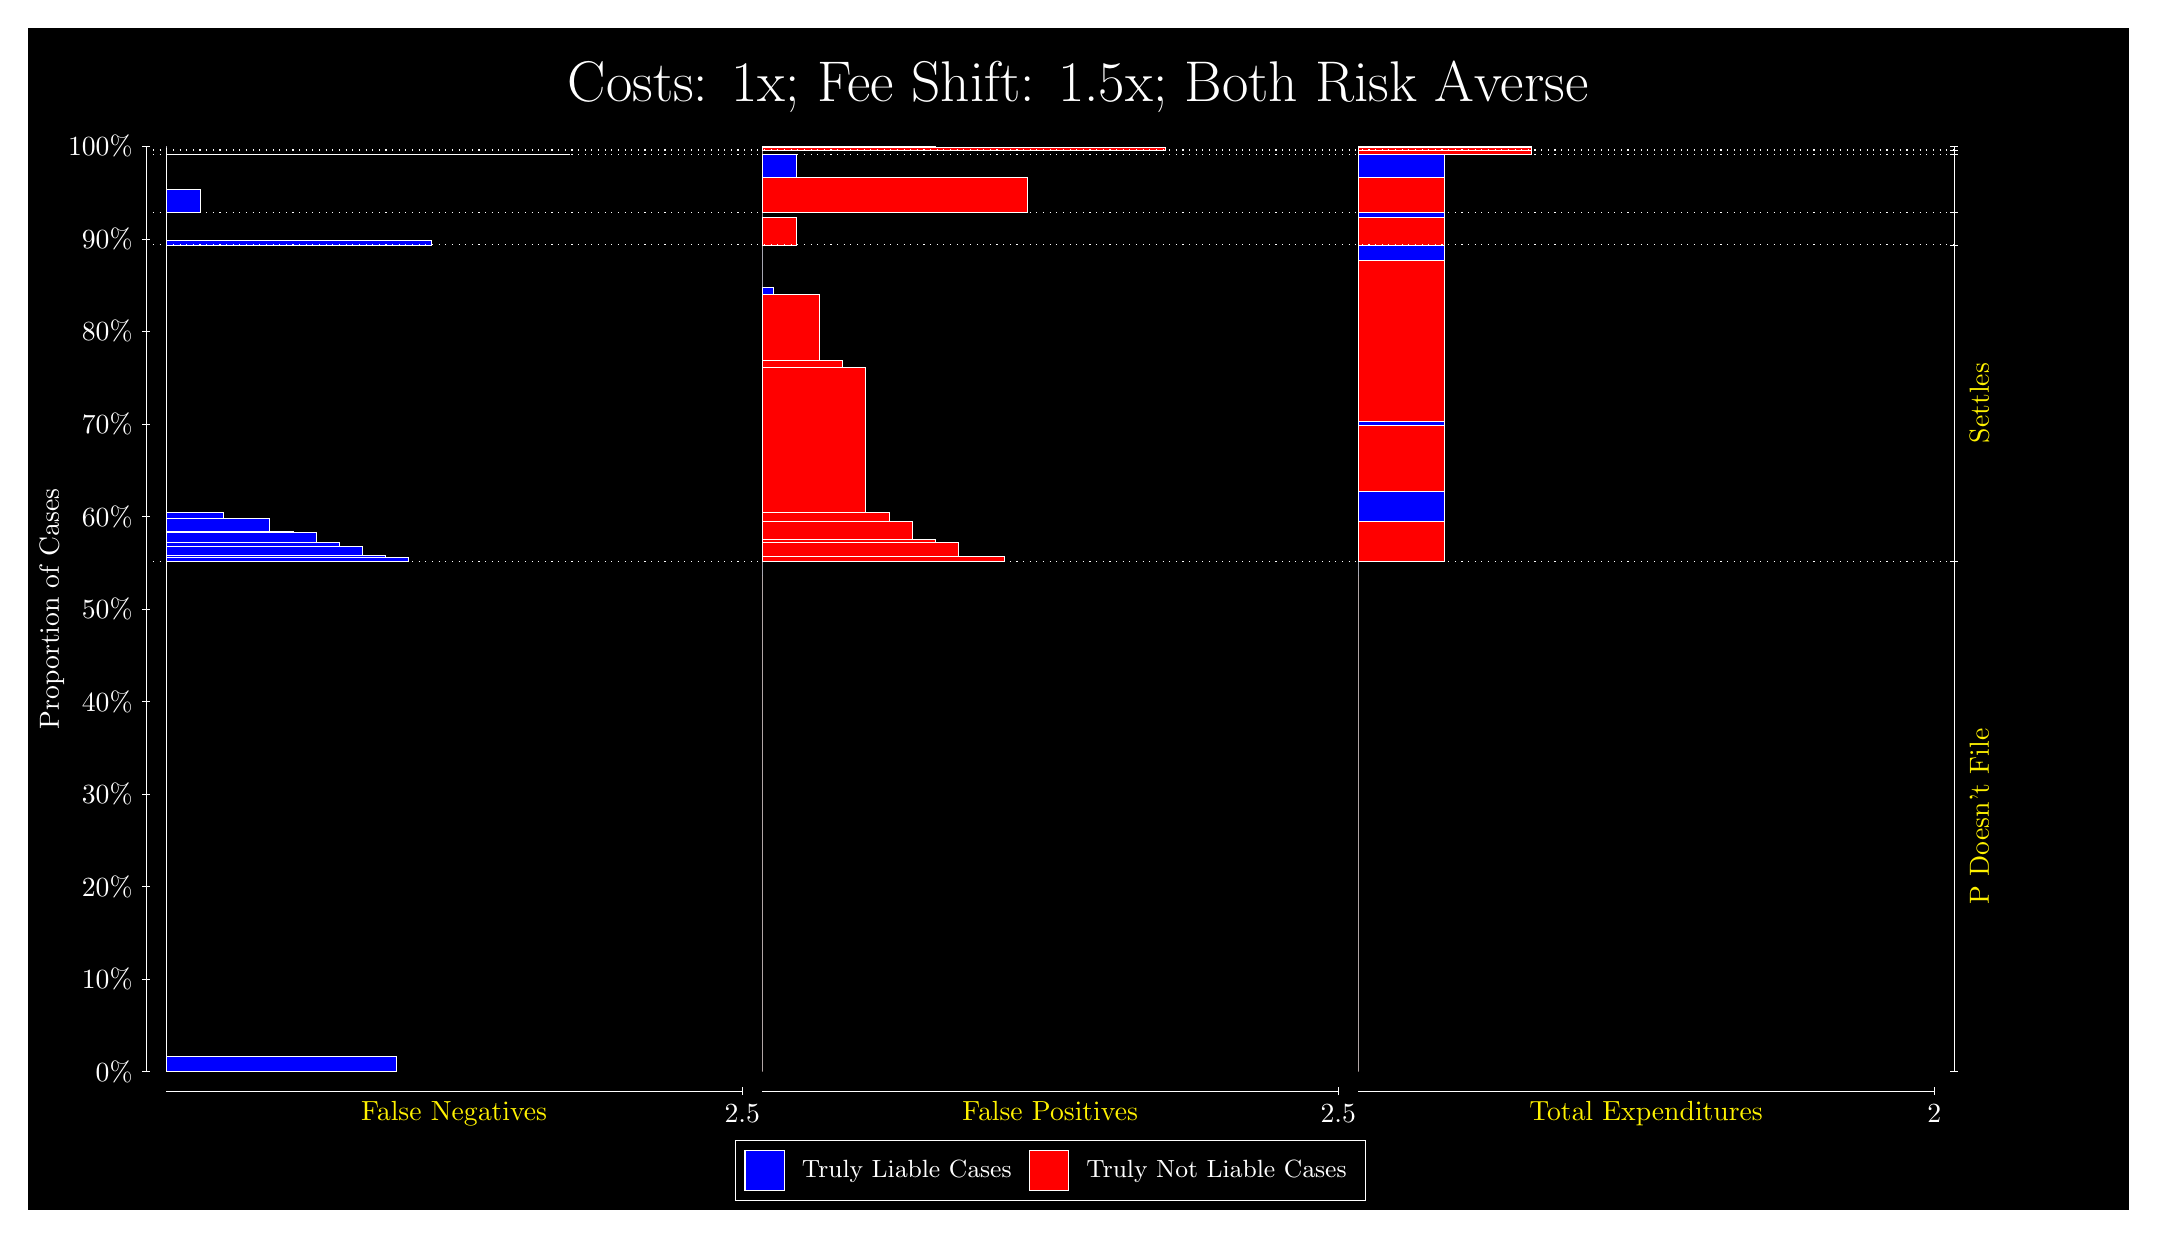
\begin{tikzpicture}
\draw[fill=black] (0,0) rectangle (26.667,15);
\draw[text=white] (0,13.5) rectangle (26.667,15) node[midway] {\huge Costs: 1x; Fee Shift: 1.5x; Both Risk Averse};
\draw[white, very thin] (1.5,1.75) -- (1.5,13.5);
\node[rotate=90, text=white, anchor=center] at (0.3, 7.625) {Proportion of Cases};
\draw[white, very thin] (1.45,1.75) -- (1.55,1.75);
\node[text=white, anchor=east] at (1.45, 1.75) {0\%};
\draw[white, very thin] (1.45,2.925) -- (1.55,2.925);
\node[text=white, anchor=east] at (1.45, 2.925) {10\%};
\draw[white, very thin] (1.45,4.1) -- (1.55,4.1);
\node[text=white, anchor=east] at (1.45, 4.1) {20\%};
\draw[white, very thin] (1.45,5.275) -- (1.55,5.275);
\node[text=white, anchor=east] at (1.45, 5.275) {30\%};
\draw[white, very thin] (1.45,6.45) -- (1.55,6.45);
\node[text=white, anchor=east] at (1.45, 6.45) {40\%};
\draw[white, very thin] (1.45,7.625) -- (1.55,7.625);
\node[text=white, anchor=east] at (1.45, 7.625) {50\%};
\draw[white, very thin] (1.45,8.8) -- (1.55,8.8);
\node[text=white, anchor=east] at (1.45, 8.8) {60\%};
\draw[white, very thin] (1.45,9.975) -- (1.55,9.975);
\node[text=white, anchor=east] at (1.45, 9.975) {70\%};
\draw[white, very thin] (1.45,11.15) -- (1.55,11.15);
\node[text=white, anchor=east] at (1.45, 11.15) {80\%};
\draw[white, very thin] (1.45,12.325) -- (1.55,12.325);
\node[text=white, anchor=east] at (1.45, 12.325) {90\%};
\draw[white, very thin] (1.45,13.5) -- (1.55,13.5);
\node[text=white, anchor=east] at (1.45, 13.5) {100\%};

\draw[white, very thin] (24.457,1.75) -- (24.457,13.5);
\draw[white, very thin] (24.407,1.75) -- (24.507,1.75);
\node[anchor=west] at (24.407, 1.75) {};
\draw[white, very thin] (24.407,8.2309) -- (24.507,8.2309);
\node[anchor=west] at (24.407, 8.2309) {};
\draw[white, very thin] (24.407,12.248) -- (24.507,12.248);
\node[anchor=west] at (24.407, 12.248) {};
\draw[white, very thin] (24.407,12.661) -- (24.507,12.661);
\node[anchor=west] at (24.407, 12.661) {};
\draw[white, very thin] (24.407,13.4) -- (24.507,13.4);
\node[anchor=west] at (24.407, 13.4) {};
\draw[white, very thin] (24.407,13.453) -- (24.507,13.453);
\node[anchor=west] at (24.407, 13.453) {};
\draw[white, very thin] (24.407,13.5) -- (24.507,13.5);
\node[anchor=west] at (24.407, 13.5) {};

\draw[white, very thin, fill=blue] (1.75,1.75) rectangle (4.6775,1.9376);
\draw[white, very thin, fill=red] (1.75,1.9376) rectangle (1.75,8.2309);
\draw[white, very thin, fill=blue] (1.75,8.2309) rectangle (4.8239,8.2826);
\draw[white, very thin, fill=blue] (1.75,8.2826) rectangle (4.5312,8.3005);
\draw[white, very thin, fill=blue] (1.75,8.3005) rectangle (4.2384,8.4262);
\draw[white, very thin, fill=blue] (1.75,8.4262) rectangle (3.9457,8.4757);
\draw[white, very thin, fill=blue] (1.75,8.4757) rectangle (3.6529,8.5961);
\draw[white, very thin, fill=blue] (1.75,8.5961) rectangle (3.3602,8.6087);
\draw[white, very thin, fill=blue] (1.75,8.6087) rectangle (3.0674,8.7756);
\draw[white, very thin, fill=blue] (1.75,8.7756) rectangle (2.4819,8.8522);
\draw[white, very thin, fill=red] (1.75,8.8522) rectangle (1.75,12.248);
\draw[white, very thin, fill=blue] (1.75,12.248) rectangle (5.1167,12.307);
\draw[white, very thin, fill=red] (1.75,12.307) rectangle (1.75,12.661);
\draw[white, very thin, fill=blue] (1.75,12.661) rectangle (2.1891,12.953);
\draw[white, very thin, fill=red] (1.75,12.953) rectangle (1.75,13.4);
\draw[white, very thin, fill=blue] (1.75,13.4) rectangle (6.8732,13.404);
\draw[white, very thin, fill=red] (1.75,13.404) rectangle (1.75,13.453);
\draw[white, very thin, fill=red] (1.75,13.453) rectangle (1.75,13.488);
\draw[white, very thin, fill=blue] (1.75,13.488) rectangle (1.75,13.5);
\draw[white, very thin, fill=red] (9.3189,1.75) rectangle (9.3189,8.0433);
\draw[white, very thin, fill=blue] (9.3189,8.0433) rectangle (9.3189,8.2309);
\draw[white, very thin, fill=red] (9.3189,8.2309) rectangle (12.393,8.2895);
\draw[white, very thin, fill=red] (9.3189,8.2895) rectangle (11.807,8.4747);
\draw[white, very thin, fill=red] (9.3189,8.4747) rectangle (11.515,8.5035);
\draw[white, very thin, fill=red] (9.3189,8.5035) rectangle (11.222,8.7426);
\draw[white, very thin, fill=red] (9.3189,8.7426) rectangle (10.929,8.8578);
\draw[white, very thin, fill=red] (9.3189,8.8578) rectangle (10.636,10.691);
\draw[white, very thin, fill=red] (9.3189,10.691) rectangle (10.344,10.788);
\draw[white, very thin, fill=red] (9.3189,10.788) rectangle (10.051,11.627);
\draw[white, very thin, fill=blue] (9.3189,11.627) rectangle (9.4652,11.704);
\draw[white, very thin, fill=blue] (9.3189,11.704) rectangle (9.3189,12.248);
\draw[white, very thin, fill=red] (9.3189,12.248) rectangle (9.758,12.602);
\draw[white, very thin, fill=blue] (9.3189,12.602) rectangle (9.3189,12.661);
\draw[white, very thin, fill=red] (9.3189,12.661) rectangle (12.686,13.108);
\draw[white, very thin, fill=blue] (9.3189,13.108) rectangle (9.758,13.4);
\draw[white, very thin, fill=red] (9.3189,13.4) rectangle (9.3189,13.449);
\draw[white, very thin, fill=blue] (9.3189,13.449) rectangle (9.3189,13.453);
\draw[white, very thin, fill=red] (9.3189,13.453) rectangle (14.442,13.488);
\draw[white, very thin, fill=blue] (9.3189,13.488) rectangle (11.515,13.5);
\draw[white, very thin, fill=red] (16.888,1.75) rectangle (16.888,8.0433);
\draw[white, very thin, fill=blue] (16.888,8.0433) rectangle (16.888,8.2309);
\draw[white, very thin, fill=red] (16.888,8.2309) rectangle (17.986,8.7426);
\draw[white, very thin, fill=blue] (16.888,8.7426) rectangle (17.986,9.1192);
\draw[white, very thin, fill=red] (16.888,9.1192) rectangle (17.986,9.9586);
\draw[white, very thin, fill=blue] (16.888,9.9586) rectangle (17.986,10.01);
\draw[white, very thin, fill=red] (16.888,10.01) rectangle (17.986,12.055);
\draw[white, very thin, fill=blue] (16.888,12.055) rectangle (17.986,12.248);
\draw[white, very thin, fill=red] (16.888,12.248) rectangle (17.986,12.602);
\draw[white, very thin, fill=blue] (16.888,12.602) rectangle (17.986,12.661);
\draw[white, very thin, fill=red] (16.888,12.661) rectangle (17.986,13.108);
\draw[white, very thin, fill=blue] (16.888,13.108) rectangle (17.986,13.4);
\draw[white, very thin, fill=red] (16.888,13.4) rectangle (19.083,13.449);
\draw[white, very thin, fill=blue] (16.888,13.449) rectangle (19.083,13.453);
\draw[white, very thin, fill=red] (16.888,13.453) rectangle (19.083,13.488);
\draw[white, very thin, fill=blue] (16.888,13.488) rectangle (19.083,13.5);
\draw[white, dotted] (1.5,8.2309) -- (24.457,8.2309);
\draw[white, dotted] (1.5,12.248) -- (24.457,12.248);
\draw[white, dotted] (1.5,12.661) -- (24.457,12.661);
\draw[white, dotted] (1.5,13.4) -- (24.457,13.4);
\draw[white, dotted] (1.5,13.453) -- (24.457,13.453);
\draw[white, very thin] (1.75,1.5) -- (9.0689,1.5);
\node[text=yellow, anchor=north] at (5.4094, 1.5) {False Negatives};
\draw[white, very thin] (9.0689,1.45) -- (9.0689,1.55);
\node[text=white, anchor=north] at (9.0689, 1.45) {2.5};

\draw[white, very thin] (9.3189,1.5) -- (16.638,1.5);
\node[text=yellow, anchor=north] at (12.978, 1.5) {False Positives};
\draw[white, very thin] (16.638,1.45) -- (16.638,1.55);
\node[text=white, anchor=north] at (16.638, 1.45) {2.5};

\draw[white, very thin] (16.888,1.5) -- (24.207,1.5);
\node[text=yellow, anchor=north] at (20.547, 1.5) {Total Expenditures};
\draw[white, very thin] (24.207,1.45) -- (24.207,1.55);
\node[text=white, anchor=north] at (24.207, 1.45) {2};

\node[text=yellow, centered, rotate=90] at (24.777, 4.9905) {P Doesn't File};
\node[text=yellow, centered, rotate=90] at (24.777, 10.24) {Settles};





\draw (12.978300999999998,1.5) node[draw=none] (baseCoordinate) {};
\begin{scope}[align=center]
        \matrix[scale=0.5, draw=white, below=0.5cm of baseCoordinate, nodes={draw}, column sep=0.1cm]{
            \node[rectangle, draw, minimum width=0.5cm, minimum height=0.5cm, fill=blue] {}; &
            \node[draw=none, font=\small, text=white] (B) {Truly Liable Cases}; &
            \node[rectangle, draw, minimum width=0.5cm, minimum height=0.5cm, fill=red] {}; &
            \node[draw=none, font=\small, text=white] (B) {Truly Not Liable Cases}; \\
            };
\end{scope}

\end{tikzpicture}
\end{document}